\documentclass[a4paper]{article}
\usepackage[polish]{babel}
\usepackage[cp1250]{inputenc}
\usepackage[T1]{fontenc}
\usepackage[dvips]{graphicx}
\usepackage{colortbl}

\pagestyle{headings}
\textwidth      15.5cm
\oddsidemargin    .1cm
\evensidemargin   .1cm

\begin{document}

\thispagestyle{empty}

\begin{minipage}{5cm}

\includegraphics[scale=0.7]{salomon.eps}
\end{minipage}
\begin{minipage}{10cm}
\begin{center}
{\Large Salomon\\
System przetwarzania wiedzy\\}
\end{center}
\end{minipage}

\vspace*{0.5cm}

\hrulefill

\vspace*{1cm}


\begin{flushright}
{\Large \emph{Vision, ver 1.1} }
\end{flushright}

%\vspace{7cm}

\begin{flushleft}
{ \Large Historia wersji }\[\]
\begin{tabular}{|p{2.5cm}||p{1.5cm}|p{6cm}|p{3.5cm}|}
  \hline
  Data & Wersja & Opis & Autor \\
  \hline \hline
  17.05.2005 & 1.0 & utworzenie & \\
  \hline
\end{tabular}
\end{flushleft}

\newpage

\section{Wprowadzenie}
Celem dokumentu SAD jest sprecyzowanie architektury systemu uwzgl�dniaj�cej now� warstw� -- \emph{Solution}, pozwalaj�cej na po��czenie z zewn�trznymi bazami danych.

\section{Architektura}

\subsection{Model logiczny}
diagramy dla Solutiona, klasy, pakiety itp

\subsection{Model implementacyjny}
nowe moduly itp, diagramy Salomon->Baza, Salomon->Pluginy (?)

\subsection{Model danych}

Do modelu bazy danych zostanie dodana nowa tabela \emph{Solutions}.
Zawiera� b�dzie nast�puj�ce pola:
\begin{itemize}
	\item SOLUTION\_ID -- unikalny identyfikator
	\item SOLUTION\_NAME -- nazwa
	\item SOLUTION\_INFO -- kr�tki opis
	\item HOSTNAME -- nazwa hosta, na kt�rym znajduje si� dana baza danych
	\item DB\_PATH -- �cie�ka do bazy na tym ho�cie
	\item USERNAME -- login do bazy danych
	\item PASSWD -- has�o
	\item C\_DATE -- data utworzenia wpisu
	\item LM\_DATE -- data ostatniej modyfikacji
\end{itemize}

Powi�zania z pozosta�ymi tabelami przedstawia poni�szy rysunek (Rys \ref{fig:salomon_db}):

\begin{figure}[ht]
	\centering
		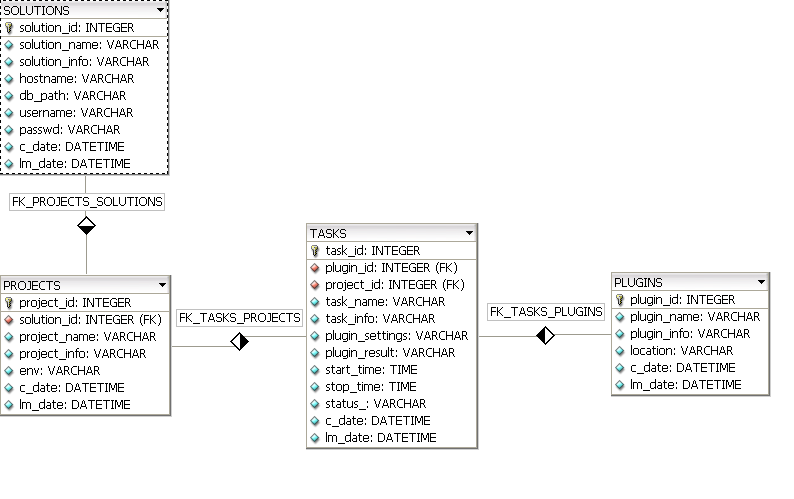
\includegraphics[width=1.00\textwidth]{../documentation/img/concept/salomon_db.png}
	\label{fig:salomon_db}
\end{figure}


\section{Model architektoniczny}
lokalizajca plikow kontfiguracyjnych itp

\begin{figure}[htbp]
	\centering
		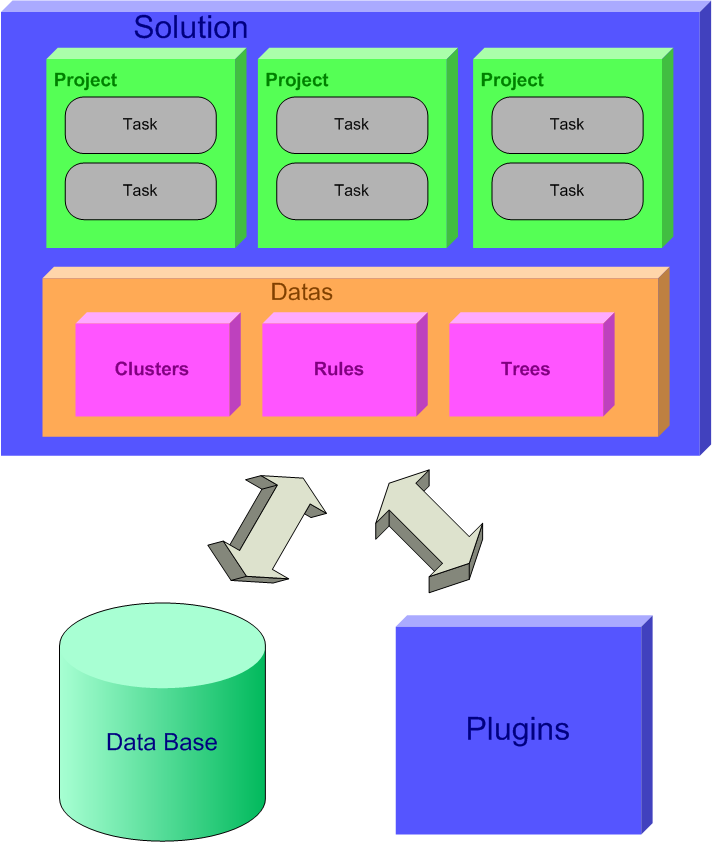
\includegraphics[width=1.00\textwidth]{img/solution.png}
	\caption{Solution}
	\label{fig:solution}
\end{figure}


\section{Troche o C2}

\end{document}

